\section{SaUCy}
\label{sec:saucy}

Using ILC, we build a concrete, executable implementation of a barebones UC
framework, dubbed SaUCy. Then, we demonstrate the versatility of SaUCy in three
ways:
\begin{enumerate}[leftmargin=*]
\item We define a protocol composition operator and its associated composition theorem.
\item We walk through an instantiation of UC commitments.
\item We use ILC's type system to reason about ``reentrancy,'' a subtle definitional issue in UC that has only recently been studied.
\end{enumerate}


%\begin{figure}
%  \centering
%  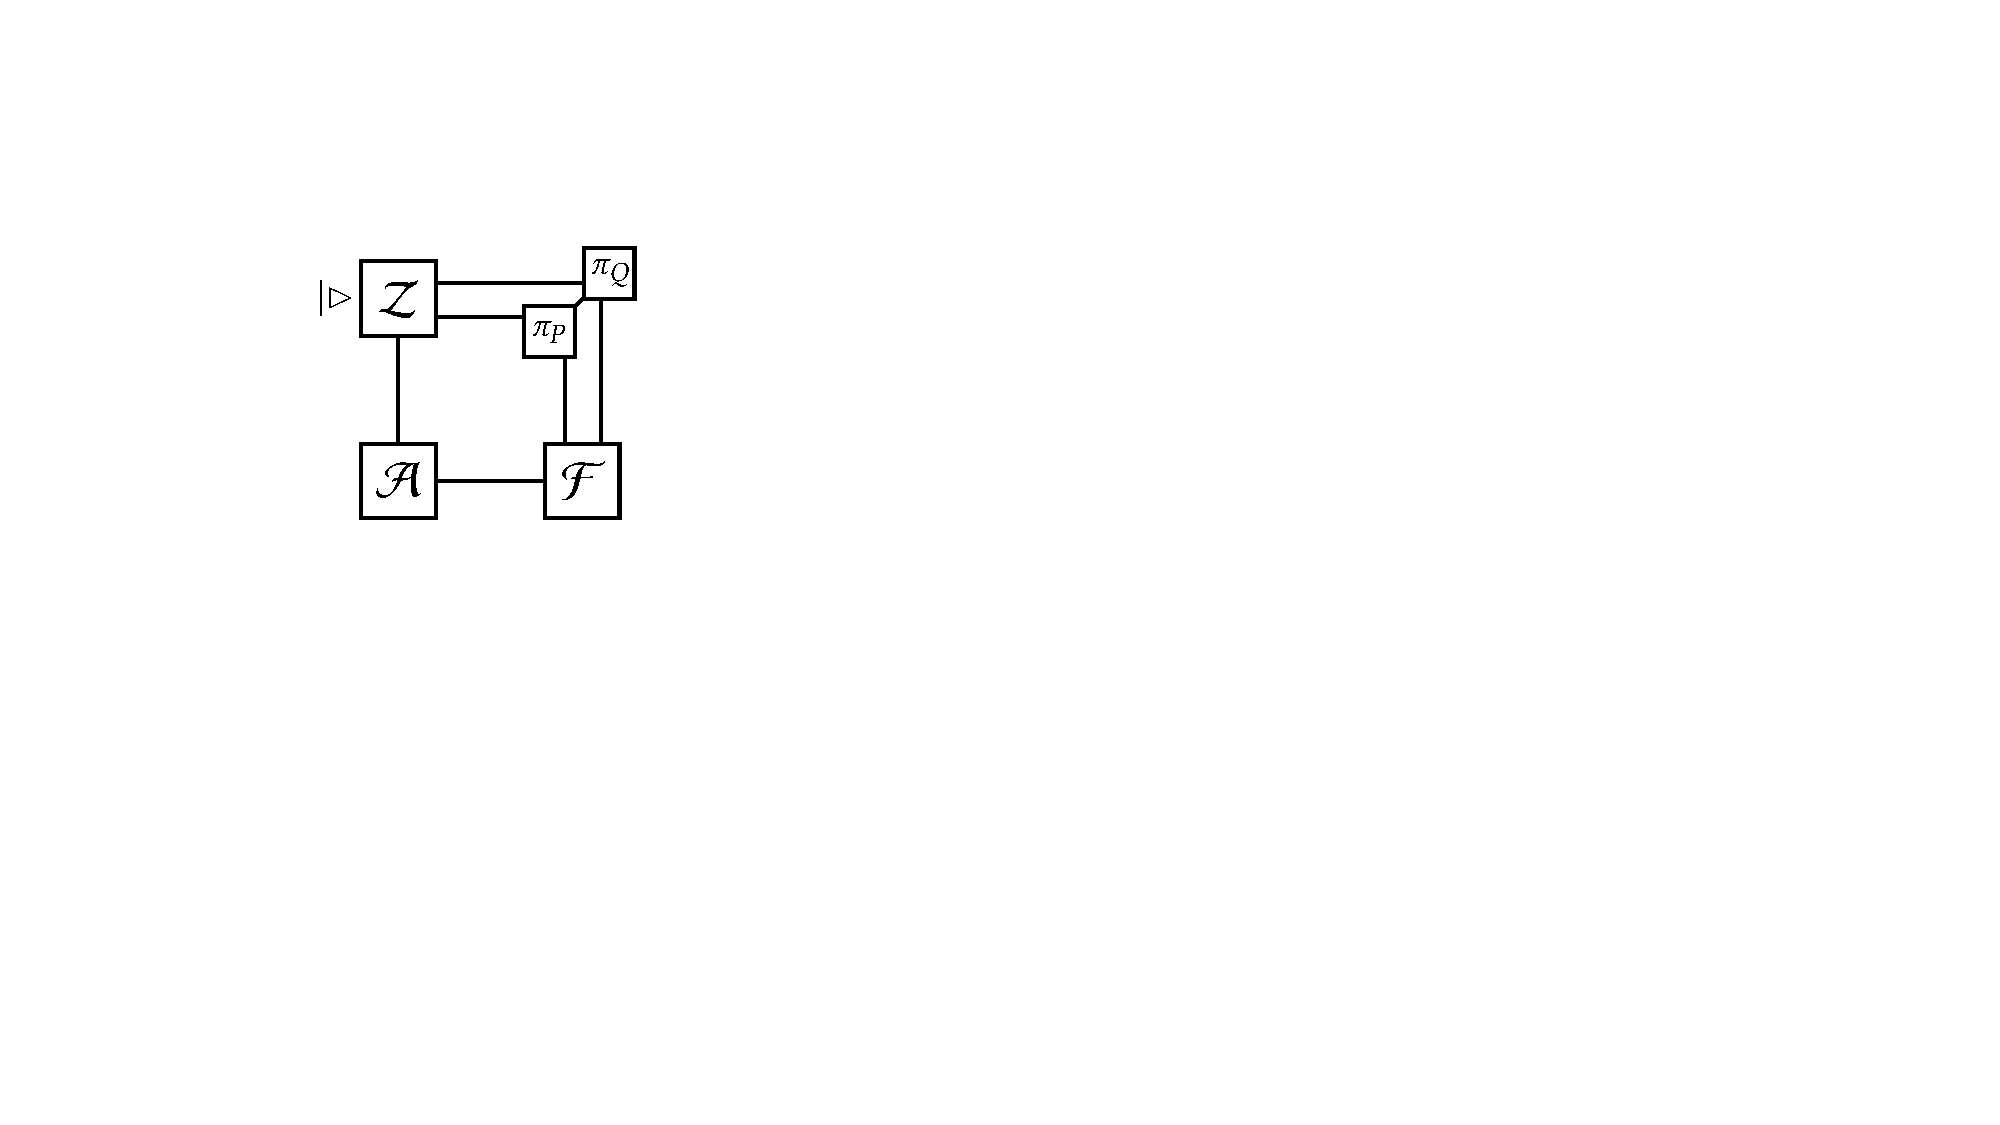
\includegraphics[width=0.4\linewidth]{graphics/execUC}
%  \caption{UC execution.}
%  \label{fig:execUC}
%\end{figure}


\subsection{Probabilistic Polynomial Time in ILC}
\label{subsec:ppt}
The goal of cryptography reduction is to relate every bad event in a protocol to a \emph{probabilistic polynomial time computation} that solves a hard problem.
The ILC typing rules do not guarantee termination, let alone polynomial time normalization, so we must tackle this in metatheory.
Also, since ILC is effectively deterministic (confluent), we will need to express random choices some other way.
To meet these needs we define a judgment about ILC terms that take a security parameter and a  stream of random bits.

\begin{definition}[Polynomial time normalization]
  \begin{comment}
  Consider a term \textsf{e} with the type
  \[\emptyctxt ;\emptyctxt |- \mathsf{e} : \tyBang{\tyNat} \multimap \tyBang{[\tyBit]}~{\multimap}_m~\tyBang{\tyBit},\]
  where the first argument is a security parameter and the second argument is a
  random bitstring.\footnote{The definition of polynomial time normalization
    applies similarly to a term \textsf{e} of type $\tyBit$ where the security
    parameter and random bitstring are free variables in \textsf{e}.} We say
  that \textsf{e} is polynomial time normalizable, written \textsf{poly(e)}, if
  for all security parameters \textsf{k} and all random bitstrings \textsf{r},
  where the length of \textsf{r} is polynomial in the security parameter
  \textsf{k}, the term \textsf{e k r} normalizes to a value \textsf{v} in a
  polynomial (in \textsf{k}) number of steps.
  \end{comment}
  The judgment that \textsf{e} is polynomial time normalizable, written \textsf{PPT e}, is defined as follows:
  \begin{mathpar}
    \Infer{ppt}
    {\wrtok ~; \emptyctxt |- e : \tyNat {->}_{\wm}\ [\tyBit] -> \mathsf{a}\\
    \forall~\mathsf{k} \in \tyNat.~\forall~r \in {[\tyBit]}^{(poly(\mathsf{k}))}.~\mathsf{e~k~r}~{->}^{poly(\mathsf{k})}~\mathsf{v}}
    {\keyword{PPT}~ \mathsf{e} }
  \end{mathpar}
  This says that if for all security parameters \textsf{k} and all bitstrings
  \textsf{r} with length polynomial in \textsf{k} the term \textsf{e~k~r} (when
  fully applied to its arguments~\todo{}) normalizes to a value \textsf{v} in
  $poly(\mathsf{k})$ steps.\footnote{Note that the normalization must be
    polynomial time for all $\mathsf{r}$, though we could have defined it to
    hold with high probability.}
\end{definition}

\begin{definition}[Value Distribution] 
  Because processes are confluent, we know that if $\mathsf{e~k~r}~{->}^{*}~\mathsf{v}$
  then the value $\mathsf{v}$ is unique.  We can therefore define the
  probability distribution ensemble
  $D(\mathsf{e}) = \{ D_{\mathsf{e,k}}\}_\mathsf{k}$
  based on a uniform distribution $U_k$ over
  $\mathsf{k}$-bit strings $\mathsf{r}$, so the distribution $D_{\mathsf{e,k}}$ is given as
\[
D_{\mathsf{e},\mathsf{k}}(\mathsf{v}) = \sum_{\mathsf{r} \in R} U_{\mathsf{k}}(\mathsf{r}), \quad \textnormal{for~} R = \{ \mathsf{r} ~|~ \mathsf{e~k~r}~{->}^{*}~\mathsf{v} \}.
\]
\end{definition}

\begin{definition}[Indistinguishability]
What remains is to define a notion of indistinguishability for value distributions. However, we need to clarify when polynomial time normalization is an assumption or a proof obligation.
  To simplify things later, we define a partial order $\mathsf{e}_1 \le \mathsf{e}_2$, which captures that $\mathsf{e}_2$ must be $\mathsf{PPT}$ if $\mathsf{e}_1$ is $\mathsf{PPT}$, and if so, that their value distributions are statistically similar.
  \begin{mathpar}
    \Infer{indist}
    {\keyword{PPT}~ \mathsf{e}_1 \implies (\keyword{PPT}~ \mathsf{e}_2 ~~\keyword{and}~~
    {D(\mathsf{e}_1) \sim D(\mathsf{e}_2)})}
    {   \qquad \mathsf{e}_1 \le \mathsf{e}_2 }
  \end{mathpar}
\end{definition}

\subsection{SaUCy Execution Model}
\label{subsec:concrete-uc}
\begingroup
\setlength\intextsep{0pt}
\setlength{\columnsep}{10pt}
\begin{wrapfigure}{R}{0.15\textwidth}
\centering
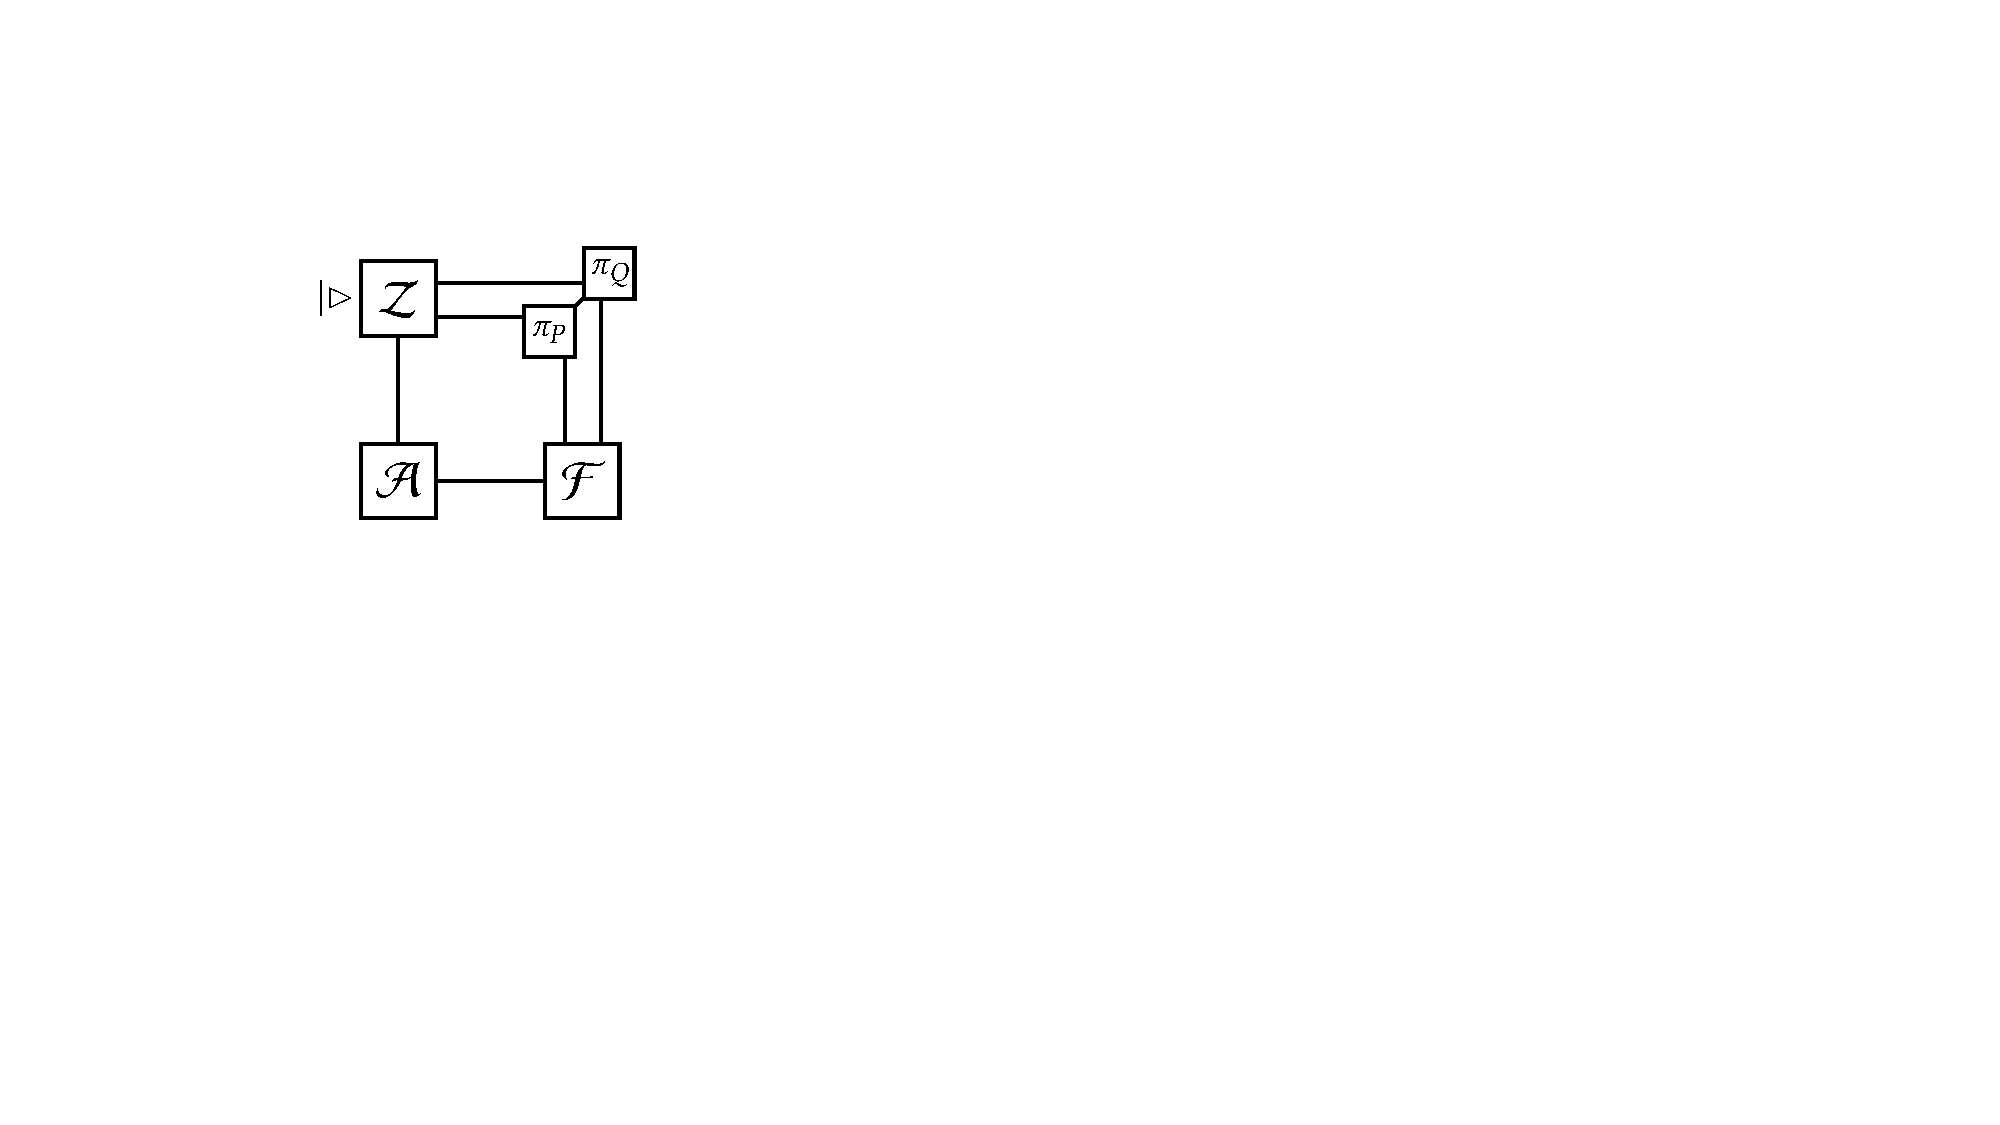
\includegraphics[width=0.15\textwidth]{graphics/execUC}
\caption{\textsf{execUC}.}
\label{fig:execUC-diagram}
\end{wrapfigure}
The implementation of SaUCy
 is centered around a definition of UC execution model in ILC.
For the most part, this just involves connecting channels as illustrated in
Figure~\ref{fig:execUC-diagram}. For demonstration, we only show
the case of two-party protocols (\`{a} la Simplified
UC~\cite{canetti2015simpler}), which will suffice for our example of
instantiating universally composable commitments.  Also, we will only aim to
show the case of \emph{static} corruptions, in which parties are corrupted at
the onset of the execution. This is in contrast to \emph{adaptive} corruptions,
in which parties can be corrupted as the execution proceeds.
\lstinputlisting[style=myilc]{listings/simp-suc.ilc}

\noindent The function \textsf{execUC} is parameterized by an environment \textsf{z},
protocol parties \textsf{p} and \textsf{q}, an adversary \textsf{a}, an ideal
functionality \textsf{f}, a security parameter \textsf{k}, a random bitstring
\textsf{r}, and a static corruption model \textsf{crupt :: Crupt}. The
\textsf{Crupt} datatype is defined below, with its variants denoting the cases
when party \textsf{p} is corrupt, party \textsf{q} is corrupt, or no party is
corrupt, respectively.
\lstinputlisting[style=myilc]{listings/crupt.ilc}
\endgroup
\noindent Some careful programming is needed to handle the cases
when the adversary sends messages on behalf of corrupted parties; this is 
captured by \textsf{wrapper} (shown in the Appendix).

Note that for space and readability, we elide channel allocation/distribution
and wrapper definitions (with ellipses). We also abbreviate the type signature
(e.g., $A_{\mathsf{z}}$ is the type of \textsf{z}). More details can be found in
the Appendix.

\begin{comment}
\begin{itemize}[leftmargin=*]
  \item \emph{Environment.} The environment's program defines interactions with
    the protocol parties and the adversary, which have different programs in the
    real world and the ideal world (see below). Its job is to distinguish which
    of the worlds it is interacting with.
  \item \emph{Protocol.} In the real world, the program of the protocol parties
    correspond to actual programs for running the protocol. In the ideal world,
    the protocol parties are simply dummy parties, which relay messages between
    the environment and the functionality.
  \item \emph{Adversary.} In the real world, the adversary is simply the dummy
    adversary, which relays messages between the environment and either the
    functionality or a corrupted party. In the ideal world, the adversary is a
    simulator, which must mimic the attack of any real world adversary, but in
    the ideal world.
  \item \emph{Functionality.} In the real world, the functionality is any
    functionality that the real world protocol makes calls to (if any). In the
    ideal world, the functionality is the specification for the protocol under
    analysis.
  \item \emph{Security parameter.} Each process is handed a security parameter
    (a natural number), and must run in a number of steps polynomial in this
    security parameter. We have more to say on this later.
  \item \emph{Corruptions.} The possible corruption models are either party
    \textsf{p} is corrupt, party \textsf{q} is corrupt, or no parties are
    corrupt, which are defined in the following datatype:
    \lstinputlisting[style=myilc]{listings/crupt.ilc}
\end{itemize}
\end{comment}

%For a real world execution, the protocol parties contain code for running the
%actual protocol under analysis, the adversary is the dummy adversary, and the
%ideal functionality is any functionality that the protocol makes calls to (if
%any). For an ideal world execution, the protocol parties are simply dummy
%parties, the adversary is a simulator, and the ideal functionality is a
%specification for the protocol under analysis. The environment has the ability
%to interact with each of the executions as they evolve. For the simulation to be
%good, the environment should not be able to distinguish which of the executions
%it is interacting with.


\subsection{Defining UC Security in ILC}
\label{subsec:uc}
The central security definition in UC is protocol emulation.  The guiding
principle is that $\pi$ emulates $\phi$ if the environment cannot distinguish between
the two protocols.  Our first attempt is the following, where $\mc{S}$ is the
simulator that translates every attack in the real world into an attack
expressed in the ideal world:
\begin{mathpar}
  \Infer{\st{emulate}}
        {\forall~\mc{Z}.~ 
         \mathsf{execUC}\ \mc{Z}\ \pi\ \mc{F}_1\ {\mathbbm{1}}_\mc{A} \le
         \mathsf{execUC}\ \mc{Z}\ \phi\ \mc{F}_2\ \mc{S}}
    {\mc{S} \entails (\pi, \mc{F}_1) \approx (\phi, \mc{F}_2)}
\end{mathpar}
To remark on a few notation choices: we make the functionality explicit, so emulation
is a relationship between protocol-functionality pairs.  Here,
$\mathbbm{1}_\mc{A}$ is the dummy adversary, which just relays messages between
the environment and the parties/functionality. We elide the standard dummy lemma that shows
this is without loss of generality; the intuition is that whatever an adversary
can do, the environment can achieve using $\mathbbm{1}_\mc{A}$.

%\[
%(\pi, \mc{F}_1) \overset{\mc{S}} \le (\phi, \mc{F}_2)
%\]
%\[
%S ~\keyword{proves}~ (\pi, \mc{F}_1) ~\keyword{emulates}~ (\phi, \mc{F}_2).
%  \]
%  Since the simulator tranlates attacks $\mc{A}$ to the real world, we treat $\mc{S}$ as a function, so $\mc{S A}$ is the ideal world adversary simulating $\mc{A}$.

%% Since emulation means that any attack on $\pi$ is also on $\phi$.
%% We have to translate \emph{attacker behaviors} of an arbitrary real world adversary $\mc{A}$ to a simulated adversary $\mc{(S~A)}$ in the ideal world.

Unfortunately this simple definition turns out to be vacuous: a degenerate
protocol $\pi$ can emulate anything simply failing to be $\keyword{PPT}$, e.g. by
diverging. To put it another way, the problem is the definition imposes a proof
obligation on the simulator $\mc{S}$ but not on $\pi$.  What we want to say is
that the \emph{real world} protocol $(\pi, \mc{F}_1)$ must be well behaved
whenever the \emph{ideal world} $(\phi, \mc{F}_2)$ is.  However, even a reasonable
protocol can result in non-PPT executions if paired with a divergent
environment.  In fact, giving a precise but composable notion of polynomial-time
for interactive processes has been an ongoing challenge in UC. In GNUC, the
approach is to define a well behaved environment, independently of its execution
context---roughly that the total size of its outgoing messages is bounded by a
polynomial, and that its running time is bounded if its total received input
size is bounded~\cite{hofheinz2015gnuc}. This notion is composable as desired,
although its use requires additional distinctions between ``invited'' and
``uninvited'' messages, which seems cluttered. RSIM makes analogous
choices~\cite{backes2007reactive}. While we think these could be equally applied to
ILC, our goal here is to provide a simpler notion.

We define protocol emulation by requiring a simulation in both directions, so every behavior in the ideal world must correspond to a behavior in the real world and vice versa.
\begin{definition}[Protocol Emulation]
  The judgment that one protocol-functionality pair $(\pi, \mc{F}_1)$  securely emulates another $(\phi, \mc{F}_2)$ (as proven the simulators $\mc{S}_\mc{R},\mc{S}_\mc{I}$) is defined as
\begin{mathpar}
  \Infer{{emulate}}
        {\forall~\mc{Z}.~ 
         \mathsf{execUC}\ \mc{Z}\ \phi\ \mc{F}_2\ \mathbbm{1}_\mc{A} \le
         \mathsf{execUC}\ \mc{Z}\ \pi\ \mc{F}_1\ \mc{S_\mc{R}} \\\\
         \ \ \ \ \ \ \ \ ~\mathsf{execUC}\ \mc{Z}\ \pi\ \mc{F}_1\ \mathbbm{1}_\mc{A} \le
         \mathsf{execUC}\ \mc{Z}\ \phi\ \mc{F}_2\ \mc{S}_\mc{I}}
    {\mc{S_\mc{R},S_\mc{I}} \entails (\pi, \mc{F}_1) \approx (\phi, \mc{F}_2)}
\end{mathpar}
\end{definition}
\noindent We remark this definition goes against the UC convention of requiring simulation in one direction only. One direction is preferable intuitively because it should be OK if the protocol is even more secure than its specification. Requiring both could be too restrictive, although we have not encountered such problem in our examples.
In any case, the benefit is this simplifies the polynomial time notion: vacuous protocols are clearly ruled out by the top condition, and both simulations are only required to be \keyword{PPT} if $\mc{Z}$ is. 

%%   \begin{mathpar}
%%   \Infer{\st{emulate}}
%%         {\forall~\mc{A}~\mc{Z}.~ \keyword{PPT}~(\mathsf{execUC}~\mc{Z}~\phi~1_\mc{A}~\mc{F}_2) => \\\\
%%   \keyword{PPT}~(\mathsf{execUC}~\mc{Z}~\pi~\mc{S_\mc{R}}~\mc{F}_1)
%% \\\\
%%          \mathsf{execUC}\ \mc{Z}\ \pi\ \mc{F}_1\ \mc{A} \le
%%          \mathsf{execUC}\ \mc{Z}\ \phi\ \mc{F}_2\ (\mc{S}~\mc{A})}
%%         {(\pi, \mc{F}_1) \overset{\mc{S}}\le (\phi, \mc{F}_2)}
%%   \end{mathpar}
  

%
%
%We therefore need to express a judgment $\keyword{Good}$ to describe environments that are well behaved in the ideal world:
%\begin{mathpar}
%  \Infer{good}
%        {\keyword{PPT}~(\mathsf{execUC}~\mc{Z}~\phi~1_\mc{A}~\mc{F}_2)}
%        {\keyword{Good}~\phi~\mc{F}_2~\mc{Z}}
%\end{mathpar}
%% To resolve this concern, we say that every \emph{benign behavior} in the ideal world must translate to. We require an additional simulator in the real world $\mc{S_\mc{R}}$      says that every benign behavior in the ideal world must correspond to a benign environment in the real world. To characteris
%% \noindent Notice that this constraint has the dummy adversary $1_\mc{A}$.
%% %, even though it is written for the ideal world, unlike in the dummy lemma.
%% This is without loss of generality in the sense that $\keyword{Good}~\phi~\mc{F}_2~Z$ implies that for any $\mc{A}$, we could have a $\mc{Z'}$ such that
%% \[
%% \mathsf{execUC}~\mc{Z} ~\phi  ~\mc{A}~\mc{F}_2 \le
%% \mathsf{execUC}~\mc{Z'}~\phi~1_\mc{A}~\mc{F}_2
%% \]


\subsection{A Composition Theorem in SaUCy}
\label{subsec:composition}

%\begin{figure}
%  \centering
%  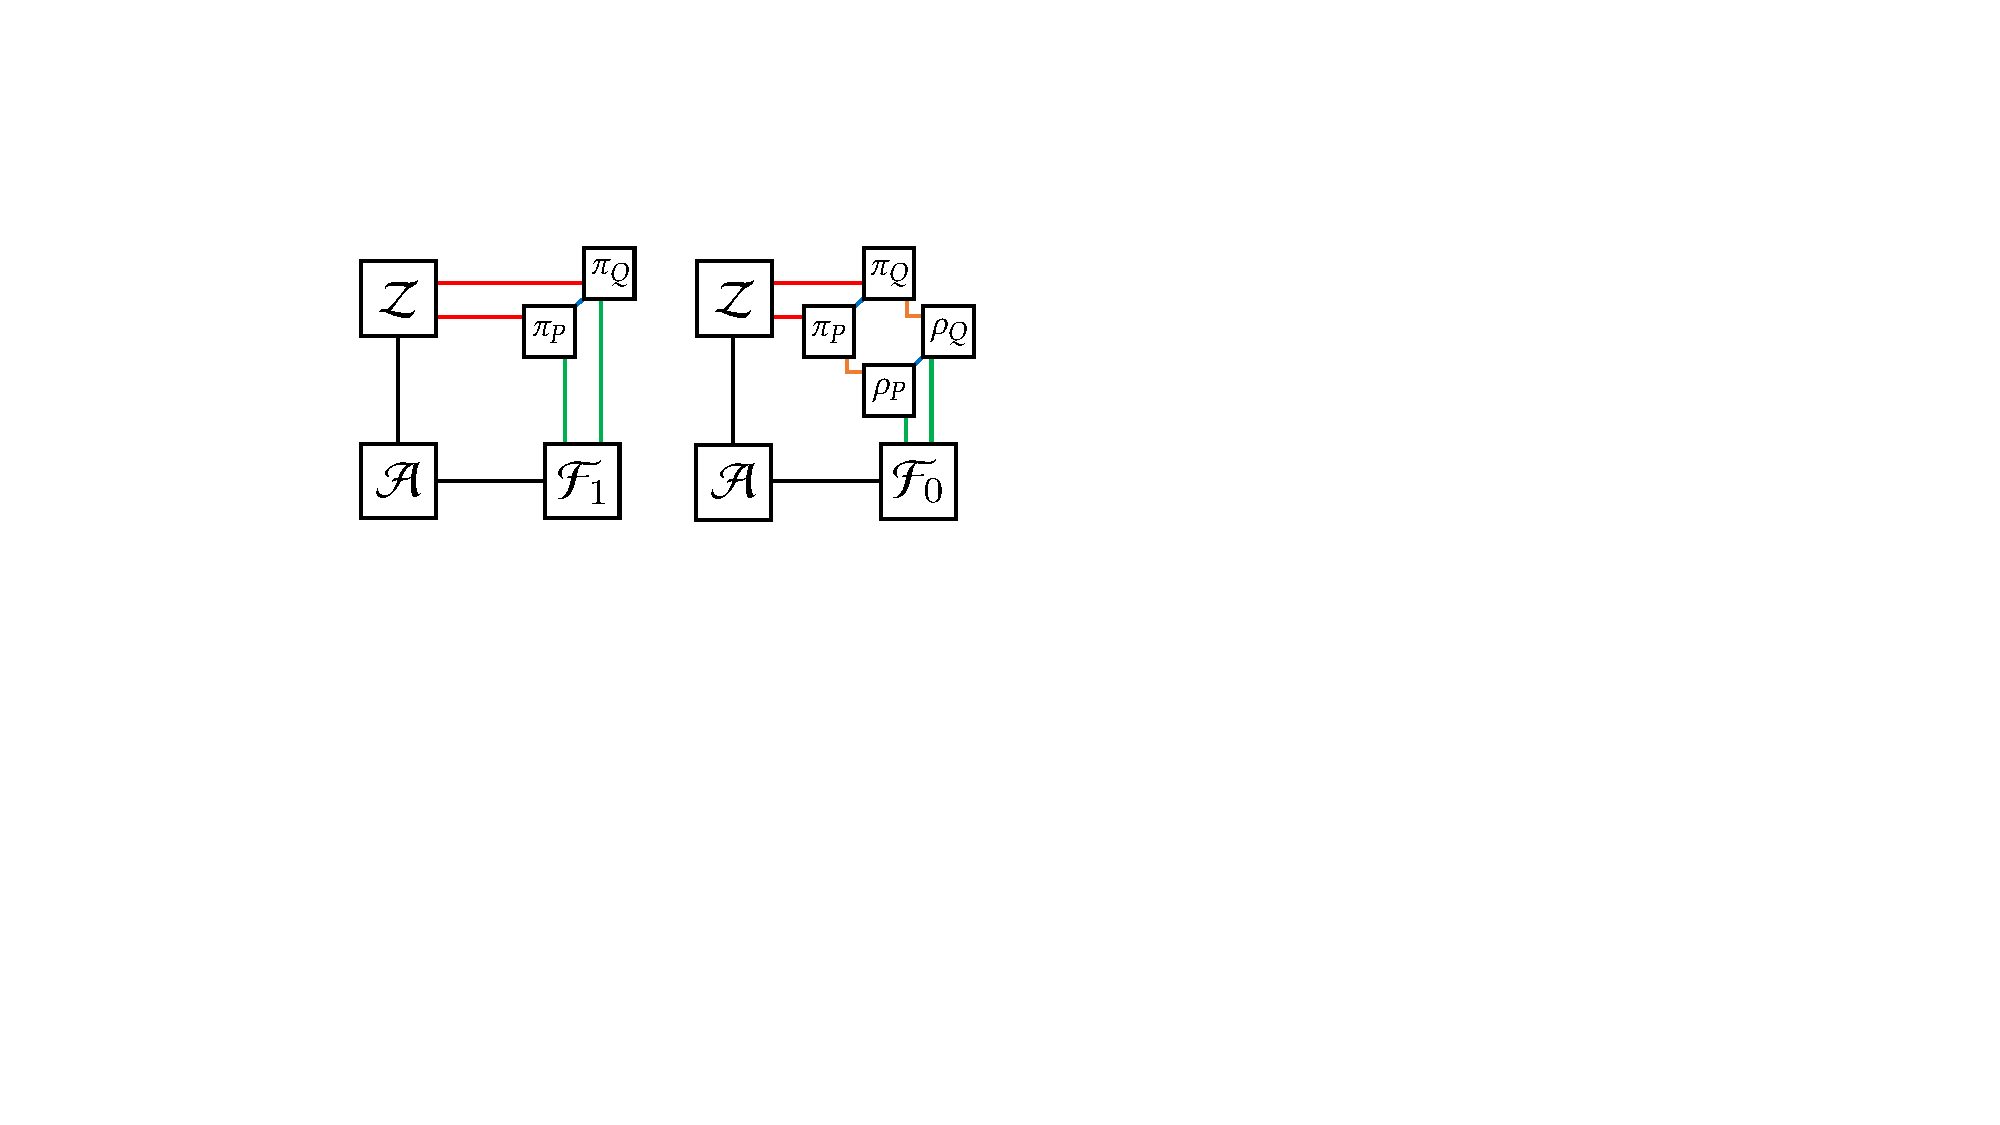
\includegraphics[width=0.75\linewidth]{graphics/protocol-composition}
%  \caption{Protocol composition diagram.}
%  \label{fig:protocol-composition}
%\end{figure}

As a first demonstration of SaUCy, we work through the development of a composition
operator, and give a theorem explaining its use.
\begin{definition}[UC realizes]
To set out, we introduce the notation of ``realizes,'' which views a protocol as a way of instantiating a specification functionality $\mc{F}_{2}$ from a setup assumption functionality $\mc{F}_1$,
%  if $\keyword(\mc{Z}, \pi, \mc{F}_0, \mc{A}_{\mathbbm{1}})$, then
%  $|- \keyword{polyUC}(\mc{Z}, \pi_{\mathbbm{1}}, \mc{F}_1, \mc{S})$, and the
  %  following statistical indistinguishability relation holds
\begin{mathpar}
  \Infer{realizes}
  {(\pi,~\mc{F}_1) \approx (\mathsf{id}_\pi, \mc{F}_2)}
  {\mc{F}_1 \yrightarrow{$\pi$} \mc{F}_2}
  \end{mathpar}
\end{definition}
\noindent where $\mathsf{id}_\pi$ is the \emph{dummy protocol}, which simply relays messages between the environment and the functionality.
This notation is convenient because it suggests a categorical approach to composition.

\begin{theorem}[Composition Theorem]
  \begin{mathpar}
  \Infer{}
  {\mc{F}_1 \yrightarrow{$\pi$} \mc{F}_2 \\ 
  \mc{F}_2 \yrightarrow{$\rho$} \mc{F}_3}
  {\mc{F}_1 \yrightarrow{$\rho \circ \pi$} \mc{F}_3}
  \end{mathpar}
\end{theorem}

\noindent The idea is that the $\rho \circ \pi$ can be defined in a natural way, where the ideal
functionality channel of $\rho$ is connected to the environment channel of $\pi$, as
illustrated and defined in Figure~\ref{fig:composition-operator}.
\begin{figure}
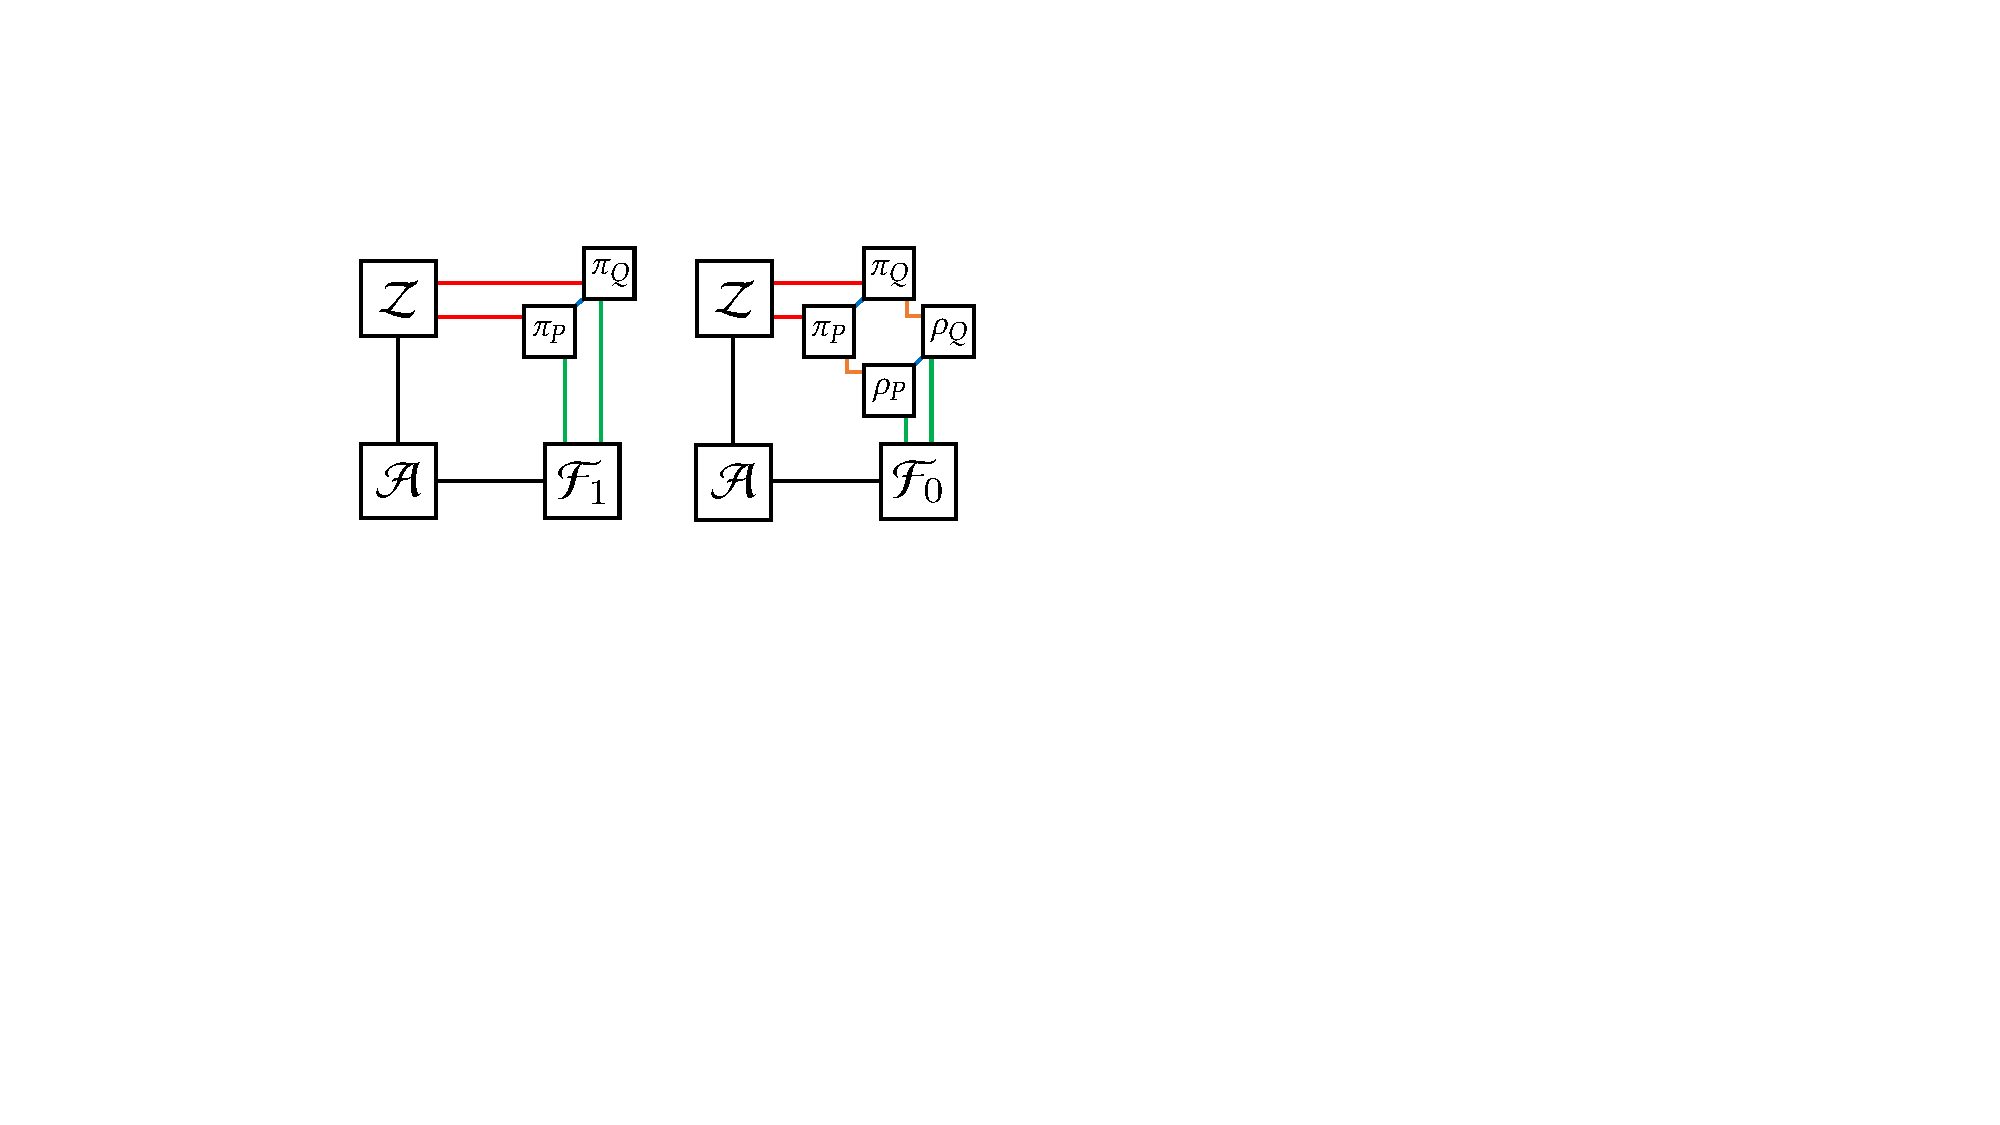
\includegraphics[width=0.75\linewidth]{graphics/protocol-composition}
\lstinputlisting[style=myilc]{listings/compose.ilc}
\caption{Protocol composition operator.}
\label{fig:composition-operator}
% The following is the nu block
  % (${\color{orange}\sf r{\rho_P}2{\pi_P}}$, ${\color{orange}\sf w{\rho_P}2{\pi_P}}$), (${\color{orange}\sf r{\pi_P}2{\rho_P}}$, ${\color{orange}\sf w{\pi_P}2{\rho_P}}$)
  % , (${\color{orange}\sf r{\rho_Q}2{\pi_Q}}$, ${\color{orange}\sf w{\rho_Q}2{\pi_Q}}$), (${\color{orange}\sf r{\pi_Q}2{\rho_Q}}$, ${\color{orange}\sf w{\pi_Q}2{\rho_Q}}$)
  % , (${\color{blue}\sf r{\rho_P}2{\rho_Q}}$, ${\color{blue}\sf w{\rho_Q}2{\rho_Q}}$), (${\color{blue}\sf r{\rho_Q}2{\rho_P}}$, ${\color{blue}\sf w{\rho_Q}2{\rho_Q}}$)		  

\end{figure}

\noindent \proof To prove the theorem we construct the simulators $S_{\mc{R},\rho} \circ S_{\mc{R},\pi}$ (respectively $S_{\mc{I},\rho} \circ S_{\mc{I,\pi}}$) in the natural way as well (given in the Appendix).
Our proof obligation is to introduce an arbitrary environment $\mc{Z}$ and conclude
\[  \keyword{execUC}~\mc{Z} ~(\rho \circ \pi)~\mc{F}_1 ~\mathbbm{1}_\mc{A}
\le \keyword{execUC}~\mc{Z} ~\mathbbm{1}_\mc{\pi} ~\mc{F}_3 ~(\mc{S}_{\mc{I},\rho} \circ \mc{S}_{\mc{I},\pi})
\]
\noindent
%
The main idea is to notice that that we can bring $\rho$ from the composed protocol into the environment as $(\mc{Z}\circ \rho)$, reflecting the fact that the environment is meant to represent arbitrary outer protocols. The following derivation completes the proof:
\begin{align*}
    &~ \keyword{execUC}~\mc{Z}~(\rho \circ \pi)~\mc{F}_1~ \mathbbm{1}_\mc{A} & \\
  = &~ \keyword{execUC}~(\mc{Z}\circ \rho)~\pi~\mc{F}_1~ \mathbbm{1}_\mc{A} &
  \textnormal{(By inspection)} \\
\le&~ \keyword{execUC}~(\mc{Z}\circ \rho)~\mathsf{id}_\pi ~\mc{F}_2~ \mc{S}_{\mc{I},\pi} & (\textnormal{From}~ \mc{F}_1 \yrightarrow{$\pi$} \mc{F}_2) \\
 = &~ \keyword{execUC}~(\mc{S}_{\mc{I},\pi}\circ \mc{Z})~\rho ~\mc{F}_2~ \mathbbm{1}_\mc{A} &  \textnormal{(By inspection)} \\
\le&~ \keyword{execUC}~(\mc{S}_{\mc{I},\pi}\circ\mc{Z})~\mathsf{id}_\pi~\mc{F}_3~\mc{S}_{\mc{I},\rho} &
(\textnormal{From}~ \mc{F}_2 \yrightarrow{$\rho$} \mc{F}_3) \\
= &~ \keyword{execUC}~\mc{Z}~ \mathsf{id}_\pi~ \mc{F}_3~ (\mc{S}_{\mc{I},\pi} \circ \mc{S}_{\mc{I},\rho}) &
\textnormal{(By inspection)}
\end{align*}
The remaining case for $\mc{S}_{\mc{R},\rho} \circ \mc{S}_{\mc{R},\pi}$ is symmetric.\qed
\begin{comment}
The following equivalence is clear:
\begin{equation}
   \keyword{execUC}~\mc{Z}~(\rho \circ \pi)~\mc{F}_1~ \mathbbm{1}_\mc{A} =
   \keyword{execUC}~(\mc{Z}\circ \rho)~\pi~\mc{F}_1~ \mathbbm{1}_\mc{A}
\end{equation}

%% (1) Notice that by code path tracing equality:
%% execUC Z φπ F1 1 =
%% execUC (Z φ) π F1 1

Next, from $\mc{F}_1 \yrightarrow{$\pi$} \mc{F}_2$ we know %
\begin{equation}
  \keyword{execUC}~(\mc{Z}\circ \rho)~\pi~\mc{F}_1 ~ \mathbbm{1}_\mc{A} \le
  \keyword{execUC}~(\mc{Z}\circ \rho)~\mathsf{id}_\pi ~\mc{F}_2~ \mc{S}_{\mc{I},\pi}
\end{equation}
%% (2) Load (A) to have
%% execUC (Z φ) π F1 1 ≤ execUC (Z φ) 1 F2 SI1

Again by equality, we can see:
\begin{equation}
  \keyword{execUC}~(\mc{Z}\circ \rho)~\mathsf{id}_\pi~\mc{F}_2 ~ \mc{S}_{\mc{I},\pi} =
  \keyword{execUC}~(\mc{S}_{\mc{I},\pi}\circ \mc{Z})~\rho ~\mc{F}_2~ \mathbbm{1}_\mc{A}
\end{equation}
%% (3) Notice that by code path tracing equality:
%% execUC (Z φ) 1 F2 SI1 =
%% execUC (SI1 Z) φ F2 1

Next, from $\mc{F}_2 \yrightarrow{$\rho$} \mc{F}_3$ we know %
\begin{equation}
   \keyword{execUC}~(\mc{S}_{\mc{I},\pi}\circ\mc{Z})~\rho~ \mc{F}_2~\mathbbm{1}_\mc{A}
\le\keyword{execUC}~(\mc{S}_{\mc{I},\pi}\circ\mc{Z})~\mathsf{id}_\pi~\mc{F}_3~\mc{S}_{\mc{I},\rho}
\end{equation}
%% (4) Load (B) to have
%% execUC (SI1 Z) φ F2 1 ≤ execUC (SI1 Z) 1 F3 SI2

Finally, again by equality:
\begin{equation}
  \keyword{execUC}~(\mc{S}_{\mc{I},\pi}~\mc{Z})~\mathsf{id}_\pi~\mc{F}_3~\mc{S}_{\mc{I},\rho} =\keyword{execUC}~\mc{Z}~ \mathsf{id}_\pi~ \mc{F}_3~ (\mc{S}_{\mc{I},\pi} \circ \mc{S}_{\mc{I},\rho})
\end{equation}
\end{comment}
%% (5) By equality:
%% execUC (SI1 Z) 1 F3 SI2 =
%% execUC Z 1 F3 (SI1 o SI2)

\paragraph{Other notions of composition.}
Our composition operator above is just a starting point.
The ``universal composition''~\cite{canetti2001universally} operator essentially multiplexes sessions identified by unique tags (\emph{session ids}), while a joint state composition theorem collapses multiple subroutines into one~\cite{canetti2003universal}.
Despite its name, development in UC often involves defining additional composition operators. 
For example, interesting composition often happens ``in the functionality''
through higher order ``wrapper''
functionalities~\cite{kosba2016hawk,katz2007universally} which we would express
through abstraction. Some security properties require a generalized notion of
ideal functionality that the environment can interact with directly. All the
above motivate the development of the ILC core calculus as a flexible
foundation; developing them in ILC is important future work. \todo{Comparison}


\subsection{Instantiating UC Commitments}
\label{subsec:example}
We now walk through an instantiation of UC commitments (\`{a} la Canetti and
Fischlin~\cite{canetti2001commitments}).  Instantiation proofs in SaUCy follow a
standard rhythm. We start with a security definition as an ideal functionality
(such as $\Func_{\textsc{Com}}$), give the protocol, construct a simulator, and
finally complete the relational analysis on paper.

UC commitments can be instantiated with standard cryptographic assumptions, for
example the RSA problem~\cite{lindell2014introduction}.  They also rely on a
``trusted setup,'' or common reference string, which are essentially public
parameters generated ahead of time (modeled as an ideal functionality
$\Func_{\textsc{crs}}$).

\paragraph{Extending ILC with cryptographic primitives.}
UC Commitments are realized from cryptographic primitives, such as trapdoor
permutations, which require extensions to ILC. The new syntactic forms are given
with their static and dynamic semantics in the Appendix.
%Figure~\ref{fig:extended-ilc}.

\paragraph{Commitment Protocol.}
The commitment protocol by Canetti and Fischlin~\cite{canetti2001commitments} is
implemented in ILC as follows:
\lstinputlisting[style=myilc]{listings/ucc.ilc}
To briefly summarize what is going on: The setup CRS functionality (given in the
Appendix) samples a random string $\sigma$ and two trapdoor pseudorandom generators (prgs $\mathsf{pk}_0, \mathsf{pk}_1$).
To commit to $b$, the committer produces a string $y$ that is the result of applying one or the other of the prgs, and if $b=1$ additionally applying xor with $\sigma$.
The intuitive explanation why this is hiding is that without the trapdoor, it is difficult to tell whether a random $4k$-bit string is in the range of either prg. To open the commitment, the committer simply reveals the preimage and the receiver checks which of the two cases applies. The intuitive explanation why this is binding is that it is difficult to find a pair $y,y\oplus\sigma$ that are respectively in the range of both prgs.

\paragraph{Defining the simulator.}
The UC proof consists of two simulators, one for the ideal world and one for the real world.
The ideal world simulator is ported directly from the UC literature~\cite{canetti2001commitments}. The non-standard real world simulator, given in the Appendix, is trivial, but necessary because our protocol emulation definition requires simulation in both directions.

The ideal world simulator generates its own ``fake'' CRS for which it stores the
trapdoors. The string $\sigma$ is not truly random, but instead is the result of
combining two evaluations of the prgs. In Figure~\ref{fig:sim-short} we show the
case that the committer P is corrupt (the other case is in the Appendix). The
simulator is activated when $\mc{Z}$ sends a message $(\mathsf{Commit}' ~ y)$;
in the real world, this is relayed by the dummy adversary to Q, who outputs
\textsf{Committed} back to the environment. Hence to achieve the same effect in
the ideal word, the simulator must send $(\mathsf{Commit}~b)$ to
$\Func_{\textsc{Com}}$. To extract $b$ from $y$, the simulator makes use of the
prg trapdoor check which one has $y$ in its range.  It is necessary to argue by
cryptographic reduction that this simulation is sound, which we describe next.

\begin{figure}
\lstinputlisting[style=myilc]{listings/sim-short.ilc}
\caption{Ideal world simulator (excerpt) for UC commitment (full version in Appendix).}
\label{fig:sim-short}
\end{figure}


\paragraph{Relational argument.}
The goal of the relational analysis is to show that an environment's output in
the real world is indistinguishable from its output in the ideal world. The
proof follows the one in Canetti and Fischlin~\cite{canetti2001commitments}.

\begin{sketch}
  Consider the following ensembles:
  \begin{align*}
    D_{\mc{R}} &= D(\mathsf{execUC~k~r~\mc{Z}~(com, rec)~fCrs~dummyA})\\
    D_{\mc{R}}' &= D(\mathsf{execUC~k~r~\mc{Z}~(com, rec)~bCrs~dummyA})\\
    D_{\mc{I}} &= D(\mathsf{execUC~k~r~\mc{Z}~(dummyP, dummyQ)~fCom~simI})
  \end{align*}
  \noindent The ensemble $D_{\mc{R}}$ is over the output of $\mc{Z}$ in a real
  world execution. The ensemble $D_{\mc{R}}'$ is similar, except $\mc{Z}$ runs
  with a bad functionality that computes fake public strings in the same way
  that the simulator does. The ensemble $D_{\mc{I}}$ is over the output of
  $\mc{Z}$ in an ideal world execution. The goal is to show that $D_{\mc{R}} \sim
  D_{\mc{I}}$.
%  
  The proof proceeds by first showing that distinguishing between $D_{\mc{R}}$
  and $D_{\mc{R}}'$ reduces to breaking the pseudorandomness of the trapdoor
  permutation (\textsf{tdp}) (hence, $D_{\mc{R}} \sim D_{\mc{R}}'$), and then by
  showing that distinguishing between $D_{\mc{R}}'$ and $D_{\mc{I}}$ also
  reduces to breaking the pseudorandomness of \textsf{tdp} (hence, $D_{\mc{R}}'
  \sim D_{\mc{I}}$). By the transitivity of indistinguishability, ${D_{\mc{R}} \sim
    D_{\mc{I}}}$.
\end{sketch}

Here, ILC's confluence property plays a critical role: It is necessary for
defining the probability ensembles $D_{\mc{R}}$, $D_{\mc{R}}'$, and
$D_{\mc{I}}$, without which we would not be able to reduce the problem of
distinguishing the real world and ideal world ensembles ($D_{\mc{R}}$ and
$D_{\mc{I}}$, respectively) to solving some computationally hard problem
(breaking the pseudorandomness of \textsf{tdp}). \todo{Check, include bCrs}

\subsection{Reentrancy in SaUCy}
\label{subsec:reentrancy}

The cryptography community has recently identified subtleties in defining UC ideal functionalities that relate to reentrancy and the scheduling of concurrent code, such that
several functionalities in the literature are ambiguous as ITMs~\cite{camenisch2016universal}.
Although concerning, these issues have no cryptographic flavor, but instead are better addressed from the PL viewpoint.
To illustrate, consider the following fragment of (untyped) ILC syntax, which allows an adversary to control the delivery schedule of messages from $P$ to $Q$ (an asynchronous channel):
\lstinputlisting[style=myilc]{listings/reentrant.ilc}
After receiving input from party $P$, it
notifies the adversary, then forks a background thread to wait for \textsf{Ok} before
delivering the message.
This introduces a race condition: suppose input message $m_1$ is sent by $P$, but then the adversary $\mathcal A$, before sending \textsf{Ok}, instead returns control to $\mathcal Z$, which passes $P$ a second input $m_2$. Now there are two queued messages. Which one gets delivered when the adversary sends \textsf{Ok}?

To resolve this paradox, notice that this fragment is untypeable in ILC.
The race condition occurs because the read channel \textsf{frA} is duplicated.
Since \textsf{frA} is linear in the function body, the function would not be typeable as intuitionistic as required by the \textsf{loop} construct.
Camenisch et al.~\cite{camenisch2016universal} identified several strategies for resolving this problem in UC, which in turn are expressible ILC. One approach is to make the process explicitly sequential, such that the arrival of a second message before the first is delivered causes execution to get stuck:
\lstinputlisting[style=myilc]{listings/reentrant-seq.ilc}
Alternatively, we may discard such messages arriving out of order, returning them to sender; we express this in ILC using the external choice operator,
\lstinputlisting[style=myilc]{listings/reentrant-ignore.ilc}

Still, the observation from Camenisch~\etal~\cite{camenisch2016universal} is
that neither of the above two solutions are completely satisfactory. The
reentrancy problem arises mainly due to the exchange of metamessages, and so
their main solution is to restrict the environment/adversary. ILC provides the
ideal starting point---restrictions on metamessages could be expressed by behavior
refinements, i.e., on receiving a message on channel A, the process P must not
send a message on its other channels until sending a message on B. \todo{Check}
